\documentclass[8pt]{article}

\usepackage[margin = 2cm]{geometry}
\usepackage{graphicx}
\graphicspath{{graphics/}}
\usepackage{amssymb}
\usepackage{multirow}
\usepackage{tabularx}
\graphicspath{{graphics/}}


\title{}
\author{}
\date{}


\begin{document}
	
\begin{center}
	\Huge{\textbf{2014-AT-02-EN Railway-System}}
	
	\begin{table}[htbp]
		\begin{center}
			\begin{tabular}{|p{3cm}|p{3cm}|p{3cm}| p{3cm}| p{3cm}|}
				\hline 
				0  ----- & I:  -----  & II:  ----- & III: hard & IV: medium \\
				
			\end{tabular}
			\begin{tabular}{|p{2.48cm}|p{2.4cm}|p{2.4cm}| p{2.4cm}| p{2.4cm}| p{2.48cm} |}
				\hline 
		[X]	ALG	& $\square$ INF  & $\square$ STRUC  & $\square$ PUZ  &  $\square$ SOC  & $\square$ USE  \\
				\hline
			\end{tabular}
		\end{center}
	\end{table}
\end{center}
\vspace{-.8cm}
\normalsize{Answer Type: Multiple Choice Graphics are: self made and colorblind proof}

\begin{center}
	\hline \hline
\end{center}
		
		  \setlength{\parindent}{0cm}
		\huge{\textbf{body}}
		\begin{figure}[htbp]
			\centering
			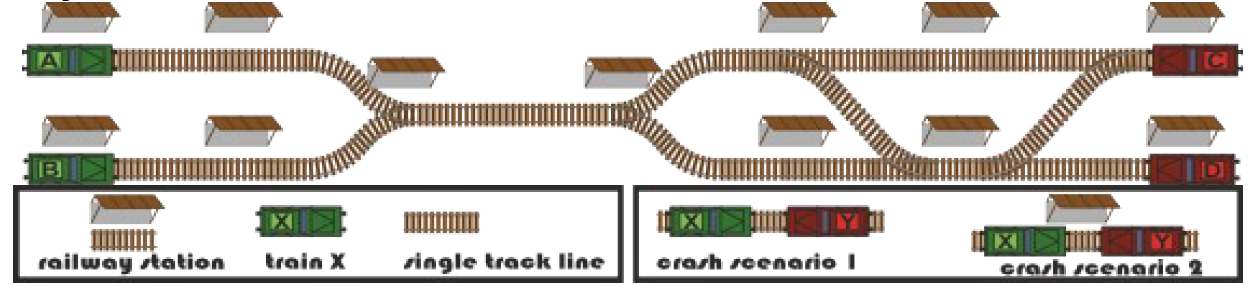
\includegraphics[scale=.5]{body.png}
		\end{figure}
	
	\large{
	In the mapped railway-system the trains A and B have to swap their positions with the
	trains C and D.
	\\*All trains will start in a schedule with an offset of one hour.
	\\*It takes one hour to cover the distance between two stations.
	\\*Once a train has started it can not be held back anymore.
	\\*The scheduler has to prevent all crash scenarios.
	\\*Scenario 1 occurs if two trains use the same single track line at the same time.
	\\*Scenario 2 occurs if two trains pull into the same station at once.
	\\*Now it's on you to create the train-schedule.}

	\setlength{\parskip}{.5cm}
    \setlength{\parindent}{0cm}
	\huge{\textbf{question}}
	
	\setlength{\parskip}{.1cm}
	\large{How does your train-schedule looks like?}





	\setlength{\parskip}{.5cm}
	\huge{\textbf{Answer}}
	
	\begin{table}[htbp]

			\newcolumntype{C}[1]{>{\centering\arraybackslash}p{#1}}
			
			\begin{tabular}{| l | C{3cm}  | C{3cm}  | C{3cm}  | C{3cm}  |}
				\hline 
				
				\multirow{3}{*}{A)} & 
\includegraphics[]{engine-A.png} &
\includegraphics[]{engine-C.png} & 
\includegraphics[]{engine-B.png} & 
\includegraphics[]{engine-D.png} \\
				& train A & train C & train B & train D\\
				\hline
				\multirow{2}{*}{B)} & 
\includegraphics[]{engine-A.png} &
\includegraphics[]{engine-B.png} & 
\includegraphics[]{engine-C.png} & 
\includegraphics[]{engine-D.png} \\
				& train A & train B & train C & train C\\
				\hline
				\multirow{2}{*}{C)} & 
\includegraphics[]{engine-A.png} &
\includegraphics[]{engine-D.png} & 
\includegraphics[]{engine-C.png} & 
\includegraphics[]{engine-B.png} \\
				& train A & train D & train C & train B\\
				\hline
				\multirow{2}{*}{D)} & 
\includegraphics[]{engine-A.png} &
\includegraphics[]{engine-C.png} & 
\includegraphics[]{engine-D.png} & 
\includegraphics[]{engine-B.png} \\
				& train A & train C & train D & train B\\
				\hline
					
				
			\end{tabular}
	\end{table}
	
\end{document}